\chapter{Background}\label{sec:background}
\begin{quote}
    In this chapter, we recapitulate the foundations which are used to build on in this work.
    In Section 2.1, we discuss the approaches to representation learning.
    In subsequent sections, we discuss an upcoming learning paradigm, self-supervised learning, the intuition and theory behind contrastive learning methods.
    In Section 2.4, we discuss convolutional neural networks for raw audio signals.
    In Section 2.5, we discuss the task of music auto tagging and their evaluation metrics.
\end{quote}


\section{Representation Learning}
% The performance of machine learning models is heavily dependent on the choice of features and representations.
% Features are often engineered using human intuition and domain knowledge of the composition of the input data, i.e., feature engineering.
% While feature engineering can greatly help to improve model performance, it is time-consuming and highlights the inability of traditional learning algorithms to identify and disentangle explanatory factors hidden in high-dimensional signals.


The goal of representation learning is to identify features that make  prediction tasks easier and more robust to the complex variations of natural data \cite{bengio2013representation}.
Supervised techniques for representation learning have now been successfully applied to a variety of tasks in the audio domain, e.g. rhythm detection, musical key recognition, chord recognition, music auto tagging, speaker identity recognition and phoneme recognition  \cite{korzeniowski_fully_2016, chen_harmony_2019, korzeniowski_end--end_2017, bock_joint_2016, pons_end--end_2017, van_den_oord_deep_2013}.

% In the unsupervised domain, generative modeling and likelihood-based models use reconstruction of the observations as the objective for learning useful representations of the data.

In unsupervised representation learning, generative modeling and likelihood-based models typically find useful representations of the data by attempting to reconstruct the observations on the basis of their learned representations \cite{goodfellow2014generative, unsupervised_gan}.
Broadly speaking, these approaches can also be considered as self-supervised representation learning: the objective is formulated in such a way that it gets supervision from the data itself.
The difference between generative approaches and self-supervised learning we like to distinguish, is that self-supervised learning aims to identify the explanatory factors of the data using an objective that is formulated with respect to the representations directly, and its goal is not to generate a faithful reproduction of the data but rather to learn useful features for (multiple) downstream tasks.
\\

\section{Self-supervised learning}
This idea of self-supervised learning has seen widespread adoption in language modeling.
Its most common task is to predict the next word, given a past sequence of words, but more auxiliary (pretext) tasks can be added to improve the language model.
For example, BERT \cite{Devlin2019BERTPO} adds two auxiliary tasks that both rely on self-generated labels to improve the bi-directional prediction of word tokens and sentence-level understanding: 1) a cloze test \cite{doi:10.1177/107769905303000401}, in which part of the tokens in each sequence is randomly masked and the model is asked to predict the missing tokens, and 2) optimizing a binary classifier on predicting whether one sequence is the next one of another sequence.
The first pretext task encourages the model to better capture the syntactic and semantic meaning of the context around a word, and the second task improves the understanding of relationships between sentences.
Building these tasks requires no manual labeling, and can therefore be scaled up to arbitrary size while there is plenty of free text available to use as training data.\\

\subsection{Formulation of pretext tasks}
In the image domain, self-supervised learning manifests itself in a similar way: one or multiple pretext tasks are formulated on a set of unlabelled images and, subsequently, the pre-trained encoder or its intermediate layers are used to fine-tune on a downstream task like image classification.
We give a short description of five different approaches.

Exemplar-CNN \cite{dosovitskiy_discriminative_2014} creates a surrogate dataset by randomly applying a sequence of transformations to `exemplary' image patches that contain large gradients, e.g., image patches that contain edges, strong textures, i.e., objects or parts of objects of interest.
Its pretext task is to classify the corresponding class of each transformed image.

An even more simple pretext task is formulated in RotNet \cite{gidaris2018unsupervised}, that proposes to use a random 2d rotation transformation as a supervisory signal to learn semantic features of an image.
The image is randomly rotated and given a class label: no rotation, $90^\circ$, $180^\circ$ or $270^\circ$, making the pretext task a 4-class classification problem.
Arguably, this forces the model to learn relationships in the semantic space of objects, i.e., to recognize the same image under different rotations, it has to learn more high-level, structural parts of the image, e.g., the relative position of a nose with respect to the eyes.
RotNet drastically reduced the gap between unsupervised and supervised feature learning in the image domain using a simple pretext task [TODO: scores here].

Another common transformation is that of colorization \cite{zhang_colorful_2016}, in which they extracted the lighting channel \textit{L} from a colored image and subsequently asked the model to predict the corresponding $a$ and $b$ color channels in CIE \textit{Lab} colorspace.

A pretext task can also be formulated as a relationship between two random patches of a single image. In \cite{doersch2015unsupervised}, they exploit the spatial context of an image as a non-exhaustive, supervisory signal.
Again given a large set of unlabeled images, random pairs of patches are extracted from each image and the network is asked to predict the position of the second patch relative to the first patch\footnote{In contrast to Exemplar-CNN, sampling is done without regard to the content of the image.}.
A $3\times 3$ grid is constructed and, given the first patch is located in the center, the model is asked to predict the location of a patch located in any of the remaining 8 positions, turning the pretext task into an 8-class classification problem.\footnote{
Interestingly, this approach quickly found a trivial solution to the problem of identifying the relative position between a pair of images: chromatic aberration.
This phenomenon arises when a lens fails to focus light at different wavelengths \cite{brewster_treatise_1835}.
Convolutional neural networks are able to localise such patches relative to the lens, which makes the objective of identifying the relative position between two patches very easy to solve.
While detailing more potential trivial solutions in the image domain is beyond the scope of this thesis, it is important to note that care must be taken for the model's ability to find trivial solutions to the problem when designing a pretext task.
In this case, the trivial solution was mitigated by shifting the green and magenta color channels to gray.
}

To conclude self-supervised learning in the image domain, \cite{noroozi_unsupervised_2016} converted aforementioned pretext task into a full $3\times 3$-grid `jigsaw puzzle', asking the model to reconstruct a sampled patch of an image after randomly shuffling all 9 sub-patches [TODO add a bit more detail why we include this].

From these series of approaches to self-supervised learning, we like to distinguish two categories of pretext tasks throughout this thesis: those that involve distortions to learn \textbf{spectral relationships} and those that extract patches to learn \textbf{spatial relationships} in data.
\\

\section{Self-supervision on Audio}
Self-supervised learning on audio brings unique challenges compared to the image domain.
Audio signals are high-dimensional, have a variable-length, and entail a hierarchical structure that is hard to infer without a supervisory signal.
It is also highly variable, given different recording conditions, voice types, instrumentation, phonemes, syllables, etc.
Work on self-supervised learning in audio was very limited at the beginning of this thesis.
While it is still very limited in the music information retrieval field, several papers were published in the speech domain.

PASE proposed a multi-task self-supervised learning approach, in which several workers each solved a self-supervised task for one neural encoder \cite{Pascual2019}.
The learned representations were proven useful for speaker identity, phoneme and emotional cue recognition.

During this thesis, PASE$+$ was published and improved on the latter method by adding random transformations to raw audio signals for more robust representations under noisy and reverberant recording environemnts \cite{Ravanelli2020}.
It outperforms both PASE and encoders trained using common audio features, like MFCC's and filter banks.

The workers in the PASE papers are small feed-forward neural networks and both solve self-supervised tasks.
Common speech features are extracted from the audio, and are used as supervisory signals for the workers.
These include regression workers that estimate log-power spectrum, MFCCs, prosody features, filter banks and their derivatives.
Other workers are simple binary classifiers trained to maximize the mutual information between representations of positive and negative samples.
The encoder and workers are jointly optimized using a loss function, which is formulated as the mean of workers' cost.


Interestingly, the self-supervised learned features are also transferable: when trained on the LibriSpeech dataset, it achieves $74.1\%$ WER on the highly challenging CHiME-5 task \cite{barker2018fifth}.
The series of transformations introduced in this paper will be further elaborated in Section \ref{sec:audio_transformations}.

VQ-Wav2Vec

Contrastive predictive coding (CPC) was introduced as a universal approach to self-supervised learning, and has been successful for speaker and phoneme classification using raw audio, among other tasks in different domains \cite{oord_representation_2019}.
It will be further detailed in Section \ref{sec:cpc}.

In music information retrieval specifically, recent advances have been made in self-supervised pitch estimation \cite{spice}, closely matching supervised, state-of-the-art baselines despite being trained without ground truth labels.
Given a segment of raw audio, it scales the pitch of the signal, converts it to the time-frequency domain using a CQT transform as input data for a ConvNet encoder, and uses the scaling factor as a supervisory signal.
To the best of our knowledge, SPICE\cite{spice} is the only (peer-reviewed) paper on self-supervised learning on audio in music information retrieval at the publication date of this thesis. We are the first to perform self-supervised learning on raw audio waveforms of musical audio, without a transformation pipeline to the time-frequency domain, and evaluate the learned representations in a musical, downstream task.

\subsection{Ideal representations}
Aforedescribed pretext tasks are designed in a way that they allow a model to learn representations that are not limited to solving the pretext task, but are also helpful in solving the downstream task when fine-tuning a classifier using the pre-trained intermediate layers as feature extractors.
Ideal feature representations should be invariant to local translations and noisy variations of the input signal while remaing sensitive to higher-level semantic information.

Put differently, the main challenge is to learn representations that effectively encode \textit{slow features} \cite{wiskott_slow_2002}, i.e., the shared information between parts of a high-dimensional signal.
Conversely, a good representation should disregard noisy, more local features.
The idea of slow features is quite intuitive for music.
We know that an audio fragment of a few seconds will share information with neighbouring fragments, e.g., the instrument(s) playing, the harmonic set of pitches or the identity of a vocalist.
 But the further into the future a model is forced to predict these features, the less of this kind of shared information is available, thereby requiring the model to infer higher-level structure.
Slow audio features span a longer temporal range (e.g., harmonic transitions or melodic contour) and are more interesting for use in downstream MIR tasks.


\subsection{Audio Augmentations}\label{sec:audio_transformations}
Earlier we distinguished two categories of pretext tasks: those that learn spectral relationships and spatial relationships.
We can extend this intuition to data augmentations, as is done in Exemplar-CNN \cite{dosovitskiy_discriminative_2014} and PASE$+$ \cite{Ravanelli2020} as to create surrogate samples or learn more robust representations respectively.

As described in the previous section, designing pretext tasks and augmentations in the audio domain brings unique challenges.
We reckon one could resort to the time-frequency domain and use spectograms or CQT-transforms and treat them as visual input data, but one could argue that aforedescribed augmentations and pretext tasks have little to do with the spectral and spatial dynamics of an audio signal, e.g., randomly flipping a spectogram or applying color jitter to a CQT-transform has hardly anything to do with the original audio signal.
We therefore describe several `spectral', i.e., acoustic augmentations that were introduced in the self-supervised speech representation learning literature \cite{Ravanelli2020} in Table \ref{tab:background_audio_augmentations}.

Augmentations of musical data are motivated by the observation that learning algorithms may generalize better and learn more robust representations when trained on samples that are perturbed \cite{Sturm2015}.
The augmentations introduced in the MUDA framework for musical data augmentations is further described in Table \ref{tab:background_music_augmentations}.
In Chapter \ref{sec:method}, more audio augmentations will be discussed, which are used in the experiments of this thesis.

\begin{fullwidth}
\begin{table}
    \centering
    \resizebox{\columnwidth}{!}{
        \begin{tabular}{lllll}\toprule
        Augmentation & Details \\\midrule
        Reverberation & Convolution with a large set of impulse responses \\
        & derived with the image method.
\\
        Additive Noise & Non-stationary noises \\
        Frequency Masking & Convolution with band-stop filters, randomly dropping\\
        & a spectrum band.
\\
        Temporal Mask & Replace a random sequence of samples with zeros.
\\ 
        Clipping & Add a random amount of saturation to simulate\\
        & audio clipping conditions.
 \\
        Overlapping & Overlap a random sample of audio to the\\
        & current audio signal.
\\
        \bottomrule
        \end{tabular}
    }
    \caption{Audio augmentations used in the speech domain to learn more robust representations using self-supervised learning methods.}
    \label{tab:background_audio_augmentations}
\end{table}
\end{fullwidth}


\begin{table}
    \centering
    \resizebox{\columnwidth}{!}{
        \begin{tabular}{lllll}\toprule
        Augmentation & Details \\\midrule
        Pitch Shift & Shift the frequency of the signal by $n \in \{ -1, 0, +1 \}$\\
        & semitones.
\\
        Time Stretch & Stretch the audio signal by a factor of\\
        & $r \in \{ -2^{\frac{1}{2}}, 1, 2^{\frac{1}{2}} \}$ \\
        Background noise & Noise under three pre-recorded conditions\\ &
        is linearly mixed with the input signal $y$, with $\alpha$ being \\
        & a random weight: $y^{\prime} \leftarrow(1-\alpha) \cdot y+\alpha \cdot y_{\text {noise }}$ \\
        Dynamic range compression & A common audio signal operation that both\\ 
        & amplifies quiet and reduces loud sounds, effectively\\
        & reducing the signal's dynamic range.
\\ 
        \bottomrule
        \end{tabular}
    }
    \caption{Musical audio augmentations from \cite{Sturm2015}}
    \label{tab:background_music_augmentations}
\end{table}




\section{Contrastive Learning}
In the following subsections, we highlight two frameworks for \textit{self-supervised} contrastive learning, currently regarded as a learning method in the self-supervised learning paradigm.
First, the generic form of the objective of these learning methods is described.


\subsection{Contrastive Loss}
The initial form of the contrastive loss function, as introduced by \cite{contrastiveloss}, runs over pairs instead of over individual samples.
While loss functions closely related to contrastive learning were introduced like metric, margin and triplet loss \cite{8014803, marginloss, chechik_large_2009}, their differences lie in the sampling strategy of positive and negative samples.
In supervised metric learning, the positive samples are chosen from the same class, while negative samples are chosen from different classes utilising hard-negative mining \cite{8014803}.
In a triplet loss function, an input sample is compared to one positive and one negative sample.
The choice of positive and negative samples in these losses are guided by the samples' corresponding labels in a supervised setting.


Contrastive losses also rely on one positive pair, which can either be picked from neighbouring patches of the anchor sample\footnote{The anchor sample and the positive sample form a positive pair}, or an augmented version of the same data point.
Different from the other loss functions, contrastive loss functions require many negative samples that are sampled from different data points.
Inherently, it is assumed this reduces the probability of a false negative.Since the loss function operates on pairs of samples, the batch of samples is often made of $2N$ data points\footnote{Very recently, BYOL proposed an online and target network model to mitigate the use of many negative samples \cite{Grill2020BootstrapYO}.
While they contributed interesting new findings, it goes beyond the scope of this thesis.}.


\begin{equation}
    \mathcal{L} = \frac{1}{2N}\sum_{i=1}^{N}\sum_{j=1}^{N} \mathbbm{1}_{[i\neq j]}\ell_{i, j}
    \label{eq:total_loss_function}
\end{equation}


\begin{equation}
    \ell_{i, j}=-\log \frac{\exp \left(\operatorname{sim}\left(z_{i}, z_{j}\right) / \tau\right)}{\sum_{k=1}^{2 N} \mathbbm{1}_{[k \neq i]} \exp \left(\operatorname{sim}\left(z_{i}, z_{k}\right) / \tau\right)}
    \label{eq:loss_function}
\end{equation}

In equations \ref{eq:total_loss_function} and \ref{eq:loss_function}, the generic form of the contrastive loss used in self-supervised learning is formulated.
We consider three types of samples\footnote{The use of the word `sample' with regard to this equation may be misleading: the $z$ terms are often embeddings of the input that passed through a parameterised function, i.e., the similarity function is formulated in latent space.} in the contrastive loss: the anchor sample, $z_i$, the positive sample, $z_j$, and the negative samples $\{ z_0 \dots z_{2N-2} \}$.
The function $\operatorname{sim}$ measures the similarity between two samples, e.g., the dot product, cosine similarity or euclidean distance.
The temperature scaling parameter $\tau$ controls the penalty of hard-negative samples.


% Intuitively, minimizing \ref{eq:loss_function} means that, for any $i$, the numerator inside the log is maximised, while the denominator is minimised.
% Since $i$ is present 


% It is insightful to consider the effects on the encoder due to minimizing Eq.
% 1. During training, for any i, the encoder is tuned to maximize the numerator of the log argument in Eq. 2 while simultaneously minimizing its denominator. The constraint that the term  is present in both the numerator and the denominator ensures that the log argument goes no higher than 1, and since Eq. 1 sums over all pairs of indices ((i, j) and (j, i)), the encoder is restricted from minimizing the denominator or maximizing the numerator without doing the other as well. As a result, the encoder learns to map similar views to neighboring representations while mapping dissimilar ones to non-neighboring ones.


\subsection{Contrastive Predictive Coding}\label{sec:cpc}

Contrastive predictive coding learns to predict representations of future observations from past observations.
For audio, it predicts representations of segments of audio in the future.
A sequential input signal $x_t$ is mapped by a non-linear encoder $g_{\mathrm{enc}}(\cdot)$ to a sequence of latent representations $h_t = g_{\mathrm{enc}}(x_t)$, while simultaneously an autoregressive model $g_{\mathrm{ar}}(\cdot)$ summarizes all encodings $h_{\leq t}$ in the latent space and maps them to a context latent representation $c_t = g_{\mathrm{enc}}(h_{\leq t})$. An visual overview of CPC is shown in Figure \ref{fig:cpc_model}.


\begin{marginfigure}[{-1cm}]
    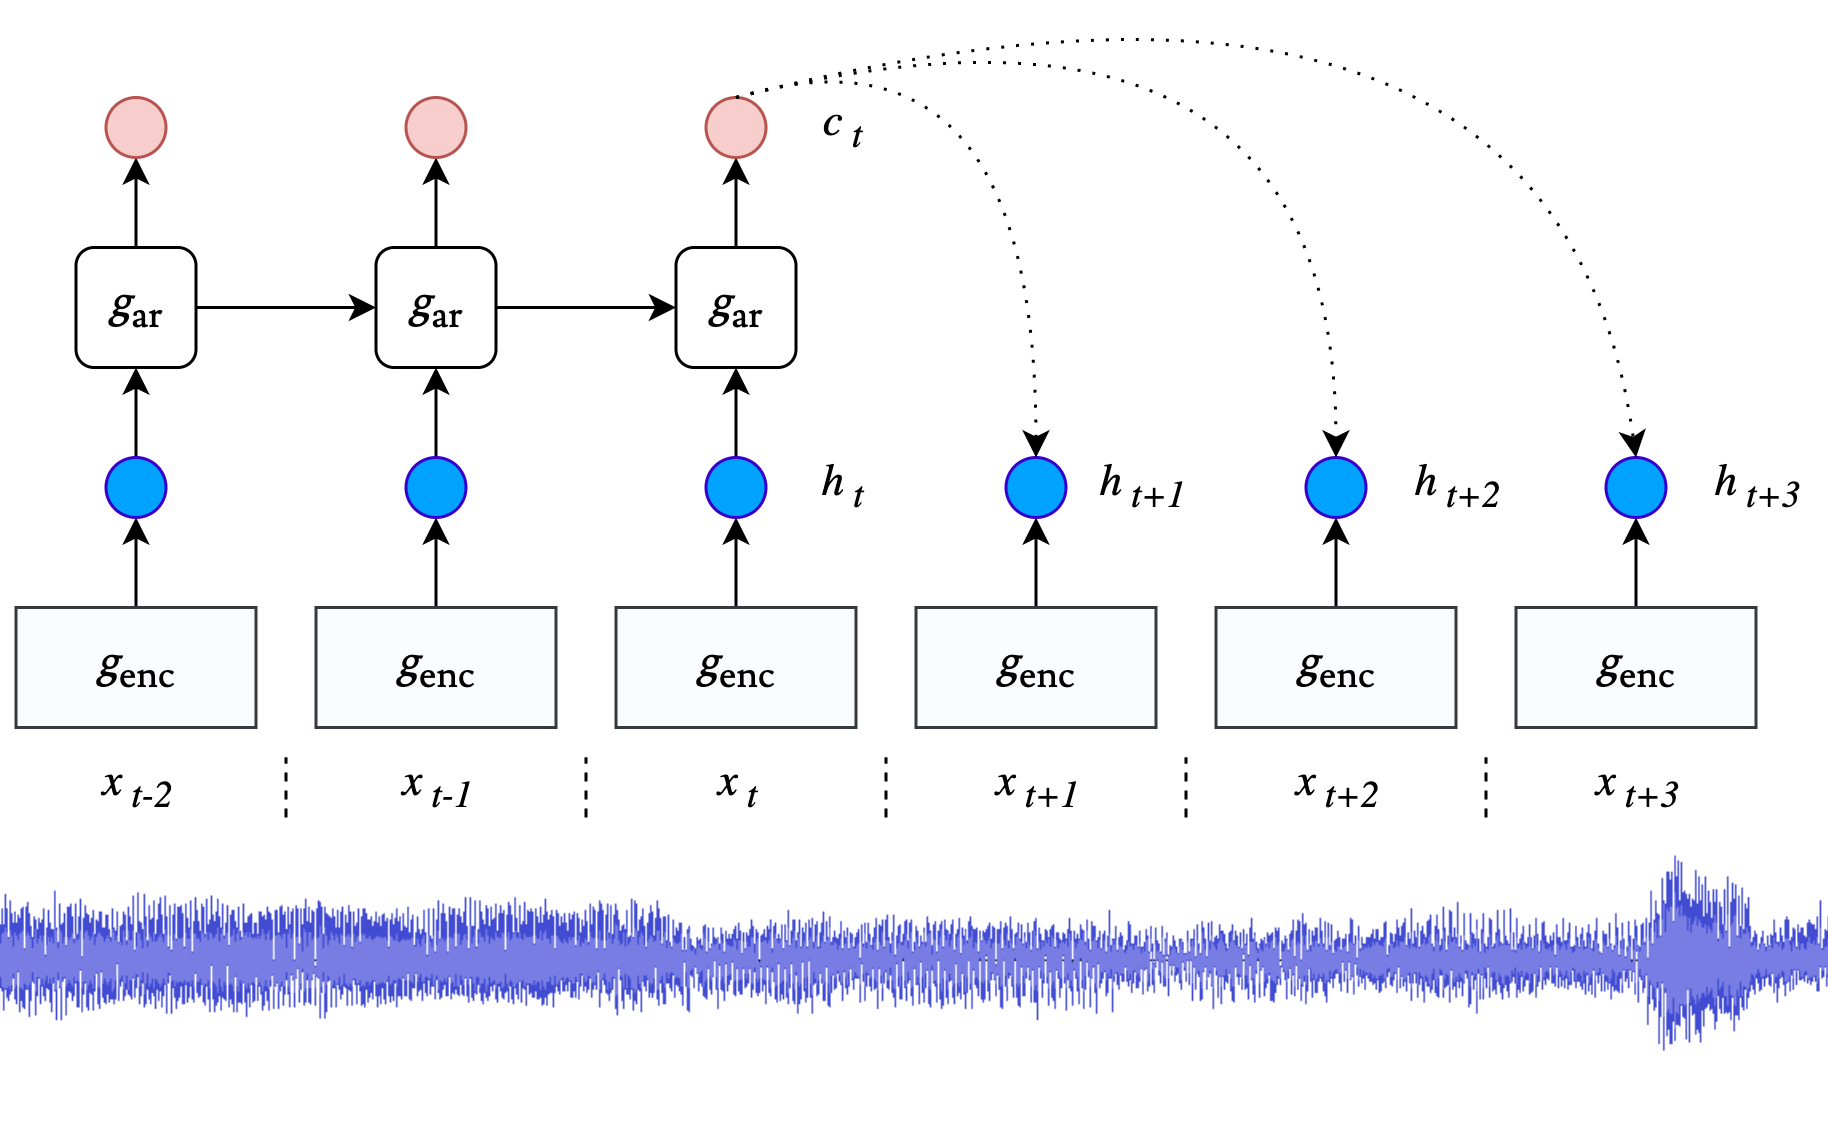
\includegraphics[width=\textwidth]{figs/cpc_model.png}
    \caption{Contrastive Predictive Coding jointly optimises two neural networks: a non-linear encoder $g_{\mathrm{enc}}$ and an autoregressor $g_{\mathrm{ar}}$, by contrasting the embeddings of temporally neighbouring patches of data using the InfoNCE loss.}
    \label{fig:cpc_model}
\end{marginfigure}

The vectors $h_t$ and $c_t$ are encoded so as to preserve maximal mutual information and to identify the shared latent variables of the original signals. The neural networks $g_{\mathrm{enc}}(\cdot)$ and $g_{\mathrm{ar}}(\cdot)$ jointly optimise the InfoNCE loss, a contrastive loss that follows the principles of noise-contrastive estimation \cite{gutmann_noise-contrastive_nodate}. Their principles are widely used in the design of self-supervised loss functions \cite{oord_representation_2019, sohn2020fixmatch, chen_simple_2020}.

Given $N$ random samples from the set of encodings $X = \{h_{t+k}, h_{j_1}, h_{j_2} \hdots h_N\}$, $k$ being the number of timesteps the encoding occurs after $c_t$ and $X$ containing one positive sample $h_{t+k}$ and $N-1$ negative samples $h_{j_{n}}$ drawn from representations of other samples in the audio and dataset, the following objective is optimised:

\begin{equation}
    \mathcal{L}_{N}=-\sum_{k} \underset{X}{\mathbb{E}}\left[\log \frac{f_{k}\left(h_{t+k}, c_{t}\right)}{\sum_{h_{j} \in X} f_{k}\left(h_{j}, c_{t}\right)}\right]
\end{equation}

Each encoding pair $(h_n, c_t)$ is evaluated using a scoring function $f(\cdot)$ to estimate how likely a given $h_n$ is the positive sample $h_{t+k}$.
CPC's formulation of the optimal solution for $f(\cdot)$ allows $-\mathcal{L}_n$ to be reformulated as a lower bound on the mutual information of representations $I(h_{t+k} | c_t)$, which also bounds the data $I(x_{t+k} | c_t)$, and is further proven by \cite{poole_variational_2019}.
For downstream tasks, both $h_t$ and $c_t$ can be used as representations for new observations $x$, depending on whether context is helpful for solving it.

Recently, the contribution of mutual information to the success of CPC has been reconsidered: its performance seems to depend largely on an inductive bias in the choice of a specialised architecture and the parameterisation of the mutual information critic \cite{Tschannen2020OnMI}.

% Contrastive predictive coding exploits this idea by learning representations that maximise mutual information among temporally neighbouring patches of data\cite{oord_representation_2019, hjelm_learning_2019}.




\subsection{SimCLR}
SimCLR is a recently proposed contrastive learning technique for learning effective representations of images in a self-supervised manner without relying on specialised architectures and powerful autoregressive modeling \cite{chen_simple_2020}.
The framework has four core components: 1) a composition of stochastic data augmentations that augment every image into two, correlated versions, 2) a ResNet encoder neural network, 3) a projector neural network and 4) a contrastive loss function, normalized temperature-scaled cross-entropy loss \cite{chen_simple_2020}.


\section{CNN's for Audio}

\subsection{SampleCNN}


\begin{table}
    \centering
    \textbf{Convolution Block} \\
    \begin{tabular}{ccccc}
        \toprule Layer & Output Size \\\hline
        & (Sequence Length $\times$ Channels) \\
        Conv & h\_in $\times$ h\_out \\
        BatchNorm & h\_out \\
        ReLU & - \\
        \bottomrule
    \end{tabular}
    \caption{Convolution block consisting of a parameterised convolution layer and batch normalisation and ReLU activation layers.}
    \label{tab:conv_block}
\end{table}

\begin{fullwidth}
    \begin{table*}[t]
        \centering
        \textbf{SampleCNN $3^9$ Model} \\
        \begin{tabular}{ccccc}
            \toprule Layer & Output Size & & Parameters & \\
            & (Sequence Length $\times$ Channels) & Kernel & Stride & Padding \\\hline
            Input & $59049 \times 1$ & 3 & 3 & 0 \\\hline
            ConvBlock & $19683 \times 128$ & 3 & 1 & 1 \\
            MaxPool & $6561 \times 128$ & 3 & 3 & 1 \\\hline
            ConvBlock & $6561 \times 128$ & 3 & 1 & 1 \\
            MaxPool & $2187 \times 256$ & 3 & 3 & 1 \\\hline
            ConvBlock & $2187 \times 256$ & 3 & 1 & 1 \\
            MaxPool & $729 \times 256$ & 3 & 3 & 1 \\\hline
            ConvBlock & $729 \times 256$ & 3 & 1 & 1 \\
            MaxPool & $243 \times 256$ & 3 & 3 & 1 \\\hline
            ConvBlock & $243 \times 256$ & 3 & 1 & 1 \\
            MaxPool & $81 \times 256$ & 3 & 3 & 1 \\\hline
            ConvBlock & $81 \times 256$ & 3 & 1 & 1 \\
            MaxPool & $27 \times 256$ & 3 & 3 & 1 \\\hline
            ConvBlock & $27 \times 256$ & 3 & 1 & 1 \\
            MaxPool & $9 \times 256$ & 3 & 3 & 1 \\\hline
            ConvBlock & $9 \times 512$ & 3 & 1 & 1 \\
            MaxPool & $3 \times 512$ & 3 & 3 & 1 \\\hline
            ConvBlock & $3 \times 512$ & 3 & 1 & 1 \\
            MaxPool & $1 \times 512$ & 3 & 3 & 1 \\\hline
            ConvBlock & $1 \times 512$ & 3 & 1 & 1 \\
            Dropout (0.5) & $1 \times 512$ & - & - & - \\\hline
            FC & 50 & - & - & - \\
            \bottomrule
        \end{tabular}
        \caption{SampleCNN $3^9$ Model, with 59049 samples (2678~ms) as input.
Each ConvBlock consists of the modules presented in Table \ref{tab:conv_block}}
        \label{tab:samplecnn_model}
    \end{table*}
\end{fullwidth}


\section{Music Tagging}

\subsection{Evaluation Metrics}

\section*{Summary}
Summary